\documentclass[journal,12pt,twocolumn]{IEEEtran}
\usepackage{cite}
\usepackage{amsmath,amssymb,amsfonts,amsthm}
\usepackage{algorithmic}
\usepackage{graphicx}
\usepackage{textcomp}
\usepackage{xcolor}
\usepackage{txfonts}
\usepackage{listings}
\usepackage{enumitem}
\usepackage{mathtools}
\usepackage{gensymb}
\usepackage{comment}
\usepackage[breaklinks=true]{hyperref}
\usepackage{tkz-euclide}
\usepackage{listings}
\usepackage{gvv}
\usepackage{braket}
\def\inputGnumericTable{}
\usepackage[latin1]{inputenc}
\usepackage{color}
\usepackage{array}
\usepackage{longtable}
\usepackage{calc}
\usepackage{multirow}
\usepackage{hhline}
\usepackage{ifthen}
\usepackage{lscape}

\newtheorem{theorem}{Theorem}[section]
\newtheorem{problem}{Problem}
\newtheorem{proposition}{Proposition}[section]
\newtheorem{lemma}{Lemma}[section]
\newtheorem{corollary}[theorem]{Corollary}
\newtheorem{example}{Example}[section]
\newtheorem{definition}[problem]{Definition}
\newcommand{\BEQA}{\begin{eqnarray}}
\newcommand{\EEQA}{\end{eqnarray}}
\newcommand{\define}{\stackrel{\triangle}{=}}
\theoremstyle{remark}
\newtheorem{rem}{Remark}
\begin{document}

\bibliographystyle{IEEEtran}
\vspace{3cm}

\title{GATE 2023 CH-58}
\author{EE23BTECH11201 - Abburi Tanusha$^{*}$% <-this % stops a space
}
\maketitle
\newpage
\bigskip

\renewcommand{\thefigure}{\theenumi}
\renewcommand{\thetable}{\theenumi}

\vspace{3cm}

\maketitle
\textbf{Question:} 
A fresh catalyst is loaded into a reactor before the start of the following catalytic reaction:
\begin{align*}
  A \rightarrow \text{Products} 
\end{align*}
The catalyst gets deactivated over time. The instantaneous activity $a(t)$, at time $t$, is defined as the ratio of the rate of reaction $-r_A(t)'$ (mol.$(g_{\text{cat}})^{-1}$hr$^{-1}$) to the rate of reaction with fresh catalyst. Controlled experimental measurements led to an empirical correlation:
\begin{align*}
 -r_A(t)' = -0.5t + 10
 \end{align*}
where $t$ is in hours.
The activity of the catalyst at $t=10$ hours is given by (rounded off to one decimal place):\\
\hfill(GATE 2023 CH)\\
\textbf{Solution:} 
\begin{table}[h!]
\centering
\resizebox{6cm}{!}{
\begin{table}[H]
    \centering
    \renewcommand\thetable{1}
    \setlength{\extrarowheight}{9pt}
    \resizebox{0.51\textwidth}{!}{
    \begin{tabular}{|c|c|c|}
    \hline
    \textbf{$r\brak{i}$} & \textbf{$p\brak{i}$} & \textbf{$k\brak{i}$} \\ \hline
    $0.06029142-0.14682007jj$ &0.88475217+0.0445749j&$2.19006287\times10^{-5}$  \\ \hline
    $0.06029142+0.14682007jj$ &0.88475217-0.0445749j&$-$  \\ \hline
    $-0.06029459+0.02518904j$ &0.94427798+0.11485352jj&$-$  \\ \hline
    $-0.06029459-0.02518904j$ & 0.94427798-0.11485352j&$-$  \\ \hline
    \end{tabular}}
    \caption{Values of $ r(i) , p(i) , k(i)$}
    \label{tab:values of r(i) , p(i) , k(i)}
    \end{table}

}
\caption{Given Parameters}
\label{tab:my_label}
\end{table}
\begin{align}
    -r_A(t)' &= -0.5t + 10 
 \end{align}   
 The rate of reaction for fresh catalyst ,at $t=0$ ;
 \begin{align}
    -r_A(0)' &= 10 \\
    -r_A(10)' &= -0.5(10) + 10 \\
              &= -5 + 10 \\
              &= 5
  \end{align}
  The activity of a catalyst at a time 't' is given by :
  \begin{align}            
    a(t) &= \frac{-0.5t+10 }{10} \\
    a(10) &= \frac{-r_A(10)'}{-r_A(0)'} \\
         &= \frac{-0.5(10)+10}{10} \\
          &= \frac{5}{10} \\
          &= 0.5
\end{align}
The activity of the catalyst at $t=10$ hours is given by $0.5$ \\

\begin{figure}[h!]
\centering
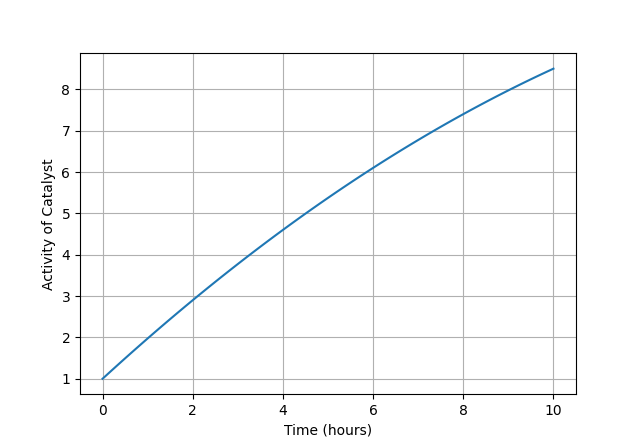
\includegraphics[width=\columnwidth]{figs/gate_plot.png}
\label{fig:plot}
\caption{Activity of catalyst vs time }
\end{figure}
\end{document}

